\documentclass{article}
\author{RustColeone}
\usepackage{amsmath}
\usepackage{amssymb}
\usepackage{amsfonts}
\usepackage{enumitem}
\usepackage{titling}
\usepackage{aligned-overset}
\usepackage{tikz}
\usepackage{wrapfig}
\usepackage{hyperref}
\usepackage{pgffor}
\usepackage{pgfplots}
\usepackage{verbatim}
\usepackage{tabularx}
%\setlength{\droptitle}{-12em}
\title{Math, Multivariable Calculus}
\setlength{\parindent}{0pt}
\newlength\tindent
\setlength{\tindent}{\parindent}
\setlength{\parindent}{0pt}
\renewcommand{\indent}{\hspace*{\tindent}}
\newcommand{\tab}[1]{
    \foreach \n in {1,...,#1}{\;\;\;\;}
}
\newcommand{\n}{$\\$}
\newcommand{\R}{\rm I\!R}
\newcommand{\parallelsum}{\mathbin{\!/\mkern-5mu/\!}}


\begin{document}
\maketitle
\newpage
\tableofcontents
\newpage
\section{Vectors}
    \subsection{Vector Calculations}
\section{Vector functions}
    \subsection{Vector Valued functions in multiple variables}
        Calculus of single variable is a study of $y=f(x)$
        \begin{align}
            y=f(x)\text{, where\;} (x\in\R)\rightarrow(f(x)\in\R)\\
        \end{align}
        However, when we are dealing with multi-variable calculus, we have: an n variable vector valued function (if $m > 1$)
        \begin{equation}
            F=
            \begin{cases}
                (x_1,\dots x_n)&\rightarrow F(x_1,\dots x_n)\\
                \text{\tab{1}}\in&\text{\tab{3}\;}\in\\
                \text{\tab{1}}\R^n&\longrightarrow\text{\tab{1}\;\;\;}\R^m\\
            \end{cases}
        \end{equation}
        where $F(x_1,\dots,x_n)=(F_1(x_1,\dots,x_n),\; F_2(x_1,\dots,x_n)\dots F_m(x_1,\dots,x_n))$\n
        The inputs and ouputs are Vectors, for example
        \begin{align}
            d(x,y) &= \sqrt{x^2+y^2}, (2 variables)\\
            (x,y)\R^2&\rightarrow(\sqrt{x^2+y^2})\R\\
            distance &= \sqrt{x^2+y^2}
        \end{align}
        \begin{center}
            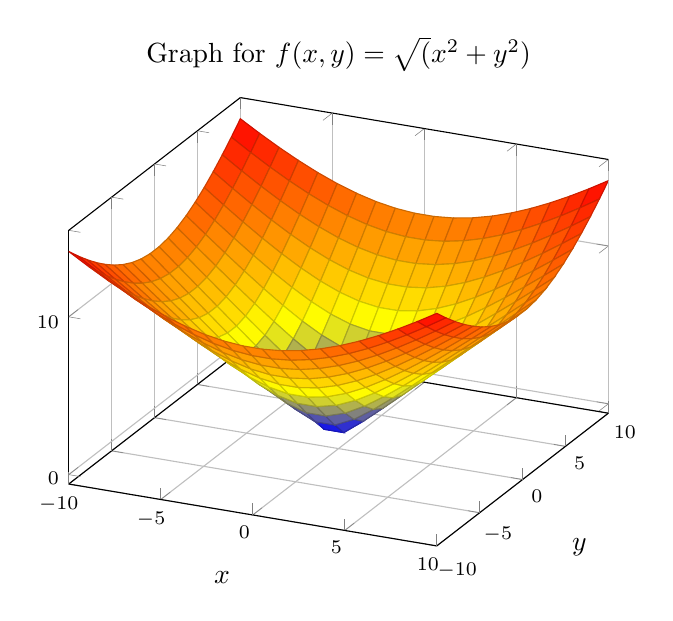
\begin{tikzpicture}
                \begin{axis} [
                    title = {Graph for $f(x,y) = \sqrt(x^2+y^2)$},
                    xtick = {-10,-5,...,10},
                    ytick = {-10,-5,...,10},
                    xlabel = $x$, ylabel = $y$,
                    ticklabel style = {font = \scriptsize},
                    grid
                ]
                \addplot3 [surf, domain=-10:10, samples=20] 
                    { sqrt(x^2 + y^2) };
                \end{axis}
            \end{tikzpicture}
        \end{center}
        \begin{center}The graph should look like a cone\end{center}
        Similarly, we can have a function that takes all the x, y and z can calculate that distance. That would however be a four dimensional plot, which we cannot plot.
        
        For a similar function, $z=x^2+y^2$\n
        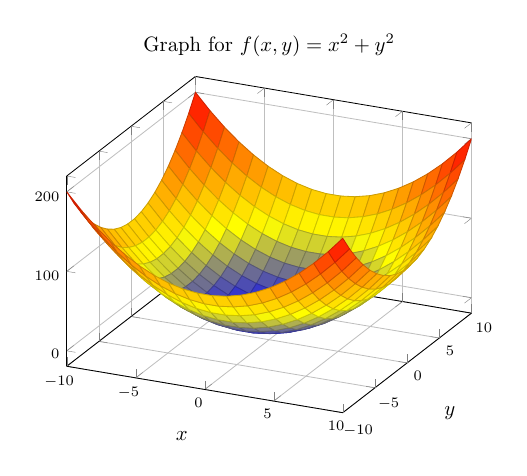
\begin{tikzpicture}[scale=0.75]
            \begin{axis} [
                title = {Graph for $f(x,y) = x^2+y^2$},
                xtick = {-10,-5,...,10},
                ytick = {-10,-5,...,10},
                xlabel = $x$, ylabel = $y$,
                ticklabel style = {font = \scriptsize},
                grid
            ]
            \addplot3 [surf, domain=-10:10, samples=20] 
                { x^2 + y^2 };
            \end{axis}
        \end{tikzpicture}
        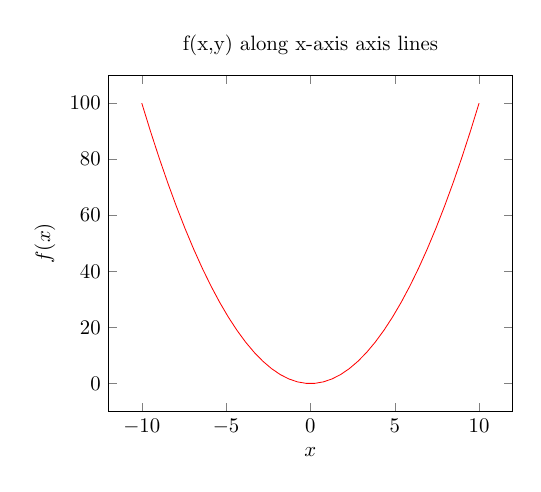
\begin{tikzpicture}[scale=0.75]
            \begin{axis}[
                title = {f(x,y) along x-axis}
                axis lines = left,
                xlabel = $x$,
                ylabel = {$f(x)$},
            ]
            \addplot [
                domain=-10:10, 
                samples=40, 
                color=red,
            ]
                {x^2};
            \end{axis}
        \end{tikzpicture}
        For another function $f(z) = (\cos{z},\sin{z})$\n
        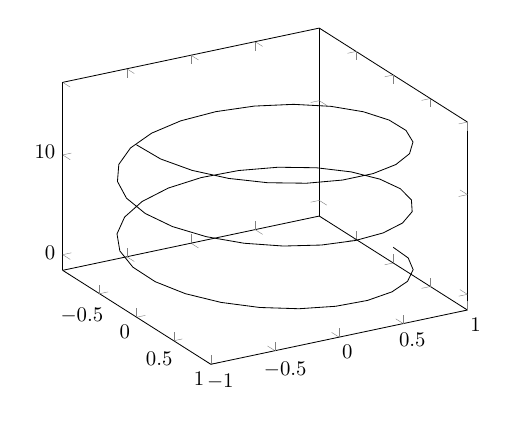
\begin{tikzpicture}[scale = 0.75]
            \begin{axis}
            [
                view={60}{30},
            ]
            \addplot3[
                domain=0:5*pi,
                samples = 60,
                samples y=0,
            ]
            ({sin(deg(x))}, {cos(deg(x))}, {x});
            \end{axis}
        \end{tikzpicture}
        \resizebox{5.5cm}{5cm}{
            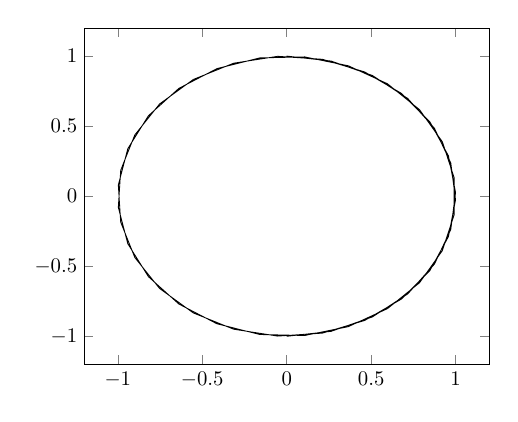
\begin{tikzpicture}[scale = 0.75]
                \begin{axis}
                [
                    view={60}{30},
                ]
                \addplot[
                    domain=0:5*pi,
                    samples = 60,
                    samples y=0,
                ]
                ({sin(deg(x))}, {cos(deg(x))});
                \end{axis}
            \end{tikzpicture}
        }
    \subsection{Limits and continuity}
        Definition:
        \begin{align}
            &\lim_{(x,y) \rightarrow (a,b)} f(x,y) = L\\
            &\text{if\;} f(x,y) \text{\;goes to L as\;}(x,y) \text{\;approaches\;}(a,b)\nonumber
        \end{align}
        \begin{center}
            \begin{tikzpicture}[scale = 0.7]
                \begin{axis}[
                    title = {continuous}
                    xlabel = $x$,
                    ylabel = {$f(x)$},
                    label = {a}
                ]
                \addplot [
                    domain=-2.5:2.5, 
                    samples=22, 
                    color=red,
                ]{-x^3};
                \end{axis}
            \end{tikzpicture}
            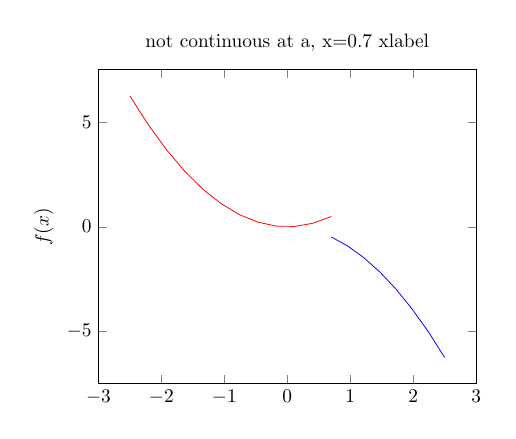
\begin{tikzpicture}[scale = 0.7]
                \begin{axis}[
                    title = {not continuous at a, x=0.7}
                    xlabel = $x$,
                    ylabel = {$f(x)$},
                ]
                \addplot [
                    domain=-2.5:0.7, 
                    samples=12, 
                    color=red,
                ]{x^2};
                \addplot [
                    domain=0.7:2.5, 
                    samples=8, 
                    color=blue,
                ]{-x^2};
                \end{axis}
            \end{tikzpicture}
            $\lim_{(x\rightarrow a^+)}f(x)=\lim_{(x\rightarrow a^-)}f(x)$, \tab{3}$\lim_{(x\rightarrow a^+)}g(x)$ DNE
        \end{center}
        Similarly, for $(x,y)\rightarrow(a,b)$ we need to look at all possible paths. If you can find 2 oaths to approach (a,b) such limits along these 2 paths are different, then the function is not continuous. For example:
        \begin{align}
            \lim_{(x,y) \rightarrow (0,0)} \frac{2xy}{x^2+y^2} &=  \text{DNE(do not exists) since:}\\
            (x,0) \rightarrow (0,0),\;\lim=\lim_{x\rightarrow0} &=\frac{0}{x^2}= 0\\
            (x,x) \rightarrow (0,0),\;\lim=\lim_{y\rightarrow0} &=\frac{2x*x}{x^2+x^2}= 1\\
            1&\neq 0\text{\;hence D.N.E.}\nonumber
        \end{align}
        Remember to take a look at all directions
        
        Definition: $f(x,y)$ continuous at $(a,b)$ if:
        \begin{enumerate}
            \item $f(x,y)$ defined at $(a,b)$
            \item $\lim_{(x,y)\rightarrow(a,b)} = f(a,b)$
        \end{enumerate}
        How to tell if a function is continuous?
        $f(x,y,z) = e^{x-z}\sin(x+yz^2)$
        \begin{enumerate}
            \item \begin{enumerate}
                    \item $f(x,y,z) = x$
                    \item $f(x,y,z) = y$
                    \item $f(x,y,z) = z all continuous$
                \end{enumerate}
            \item $f(x,y,z) = x-z$
            \item $f(x,y,z) = e^{x-z}(composition of contin.func is contin.)$
            \item $g(x,y,z) = \sin(x+yz^2)$ continuous similarly
        \end{enumerate}
        Test: $\lim_{(x,y,z)\rightarrow(0,1,-1)} = e^1\sin{(1)}$, hence continuous. A special case is when you have $\frac{f(x,y)}{g(x,y)}$, it will be continuous at (a,b) as long as $g(a,b) \neq 0$
        
        For a vector function $F(\vec{v}) = (F_1(\vec{v}),F_2(\vec{v}\dots F_m(\vec{v})$, where $\vec{v}$ is a vector or $\R^n, (x_1,x_2\dots x_n)$, is a continuous function at vector $\vec{n}$ if all its component functions are continuous at $\vec{n}$
        
        Example:
        \begin{align}
            f(x,y,z) = (e^{x+y},\;z,\;\cos(x^2-z)) \text{\;continuous everywhere}\\
            \text{since}\begin{cases}
                e^{x+y} \text{\;continuous} \\
                z \text{\;continuous} \\
                \cos(x^2-z) \text{\;continuous}
            \end{cases}
        \end{align}
    
    \subsection{Partial Derivatives}
        The derivative of a function is the rate of change along the x axis. The partial derivatives of $F(x,y)$ would be the rate of change of F as one of the axis is fixed (along one axis).
        \begin{align}
            \frac{dF(x,y)}{dx} = F_x(x,y) = \lim_{\Delta x \rightarrow 0}\frac{F(x+\Delta x,y)-F(x,y)}{\Delta x}\\
            \frac{dF(x,y)}{dy} = F_y(x,y) = \lim_{\Delta y \rightarrow 0}\frac{F(x,y+\Delta y)-F(x,y)}{\Delta y}
        \end{align}
        In order to compute the derivative, we treat all other variables as constants.
        
        Example:
        \begin{align}
            f(x,y,z) = xe^{xy}-\sin{(y^2+z^2)}\\
            \frac{df}{dx} = e^{xy}+yxe^{xy}-0=e^{xy}+yxe^{xy}\\
            \frac{df}{dy} = x^2e^{xy}-\cos{(y^2+z^2)}(2y)
            \frac{df}{dz} = 0-\cos{(y^2+z^2)}(2z)
        \end{align}
        Take a point $(a,b)$ for example
        \begin{enumerate}
            \item $\frac{df}{dx} = $ gradient of tangent at that point along x axis\n
            \item $\frac{df}{dy} = $ gradient of tangent at that point along y axis\n
            \item These two direction can span the tangent plane of f at that point
            \begin{enumerate}
                \item Tangent Vector
                \item along x direction $= (1,0,\frac{df}{dx}(a,b)) = \vec{v}$
                \item along y direction $= (0,1,\frac{df}{dy}(a,b)) = \vec{w}$
                \item Using these vectors we can find the plane's equation
            \end{enumerate}
        \end{enumerate}
        Example, find the tangent plane of $f(x,y)$ at (1,1):
        \begin{align}
            f(x,y) &= 1-x^2-2y^2\\
            f(1,1) &= z = -2, \text{\;point at\;} (1,1,-2)\\
            \frac{df}{dx} &= (1,0,-2x|_{(1,1)}) = (1,0,-2)\\
            \frac{df}{dy} &= (1,0,-4y|_{(1,1)}) = (0,1,-4)\\
            (1,0,-2)\times(0,1,-4) &= (2,4,1)\\
            2x+4y+z &= 4\text{\;a linear approximation of\;}f(x,y)\text{\;at\;}(1,1)
        \end{align}
        
        Definition of a vector function:
        \begin{align}
            F(x_1,x_2\dots,x_n) = F(\vec{x}) = (F_1(\vec{x})\dots F_m(\vec{x}))\in \R^m
        \end{align}
        Where each $F_i$ is a component function. The derivative the size $(m \times n)$ matrix of $F$(Jacobian matrix) denoted by $DF(\vec{x})$
        \begin{equation}
            DF(\vec{x}) = 
            \begin{pmatrix}
                \frac{dF_1}{dx_1} & \frac{dF_1}{dx_2} & \dots & \frac{dF_1}{dx_n}\\
                \frac{dF_2}{dx_1} & \frac{dF_2}{dx_2} & \dots & \frac{dF_2}{dx_n}\\
                \dots&\dots&\dots&\dots\\
                \frac{dF_m}{dx_1} & \frac{dF_m}{dx_2} & \dots & \frac{dF_m}{dx_n}
            \end{pmatrix}
        \end{equation}
        The function F transforms$\R^n\rightarrow\R^m$, $DF\;\R^n\rightarrow\R^m$ is a linear map, a linear approximation of F.
        
        Example:
        \begin{align}
            F(x,y,z) = (e^{x+yz},x^2+1,\sin{(y+z)},4y)
        \end{align}
        \begin{equation}
            DF(x,y,z) = 
            \begin{pmatrix}
                e^{x+yz} & ze^{x+yz} & ye^{x+yz}\\
                2x       & 0         & 0\\
                0        & \cos(y+z) & \cos(y+z)\\
                0        & 4         & 0
            \end{pmatrix}\\
            DF(1,1,2) = 
        \end{equation}
        \begin{equation}
            DF(1,1,2) = 
            \begin{pmatrix}
                e^{3} & 2e^{3} & e^{3}\\
                2     & 0      & 0\\
                0     & \cos(3)& \cos(3)\\
                0     & 4      & 0
            \end{pmatrix}
        \end{equation}
        Matrix of numbers, a linear map
        \begin{align}
            F(x,y,z) = (e^{x+yz},x^2+1,\sin{(y+z)},4y)
        \end{align}
    \subsection{Properties of Derivatives DF}
        Given two vector function F and G: $\R^n\rightarrow\R^m$ both differentiable at some point $\vec{x}$
        \begin{align}
            &D(f\pm G) = D(F) \pm D(G)\\
            &C \in \R, D(cF) = cD(F)
        \end{align}
        suppose\; $f,g:\R^n\rightarrow\R $ a function in n variables, product rule still holds
        \begin{align}
            &D(f\cdot g) = D(F)\cdot g + f\cdot D(G)
        \end{align}
        where $D(f\cdot g)$ is a $n^{th}$ dimension vector, D(f or g) is a vector function and f or g is a scalar function
        \begin{align}
            &D(\frac{f}{g}) = \frac{g\cdot D(F) - f\cdot D(G)}{g^2}\text{,\;}g(\vec{x})\neq0
        \end{align}
        
        Given two vector function $\vec{v}(t)$ and $\vec{w}(t)$: $\R\rightarrow\R^n$ so $t\rightarrow\vec{v}(t)$
        \begin{align}
            f(t) &= \vec{v}(t) \cdot \vec{w}(t) \text{scalar function}\\
            f'(t)&= \vec{v}(t)' \cdot \vec{w} + \vec{w}(t)' \cdot \vec{v}\\
            u(t) &= \vec{v}(t) \times \vec{w}(t) \text{vector function}\\
            u'(t)&= \vec{v}(t)' \times \vec{w}(t) + \vec{w}(t)' \times \vec{v}(t)\\
            \vec{v}(t) &= \langle v_1(t), v_2(t), \dots v_n(t) \rangle
        \end{align}
        Chain rule, suppose $f:\R^m\rightarrow\R^n$, $g:\R^n\rightarrow\R^p$, $g\cdot f:\R^m\rightarrow\R^p$, $\vec{x}\in\R^m$
        \begin{align}
            D(g\circ f)(\vec{x})\text{(size $p\times m$)} &= DG(F(\vec{x}))\text{(size $p\times n$)}\cdot DF\vec{x}\text{(size $n\times m$)}\\
            (g\circ f)'(x) &= g'(f(x))\cdot f'(x)
        \end{align}
        
        Example:
        \begin{align}
            f(x,y) &= (x^3 + y, e^{xy}, 2+xy) \R^2\rightarrow\R^3\\
            g(y,v,w) &= (y^2+v,uv+w^3) \R^3\rightarrow\R^2\\
            g(f(x,y)) = g\circ f &= ((x^3+y)^2+e^{xy},\;(x^3+y)e^{xy}+(2+xy)^3)
        \end{align}
        \begin{equation}
            D(g\circ f) = \begin{pmatrix}
                2(x^3+y)(3x^2) + ye^{xy}                &   2(x^3+y)+xe^{xy} \\
                \begin{pmatrix}
                    3x^2e^xy+(x^3 + y)ye^{xy}\\+3(2+xy)^2y
                \end{pmatrix}    &   
                \begin{pmatrix}
                    e^{xy}+(x^3+y)xe^{xy}\\+3(2+xy)^2x
                \end{pmatrix}
            \end{pmatrix}
        \end{equation}
        \begin{equation}
            DG = \begin{pmatrix}
                2u  &   1   &   0\\
                v   &   u   &   3w^2
            \end{pmatrix}
        \end{equation}
        \begin{align}
            (g\circ f)'(x) &= g'(f(x))\cdot f'(x)
        \end{align}
        \begin{equation}
            DG = \begin{pmatrix}
                2(x^3+y)  &   1       &   0\\
                e^{xy}    &   x^3+y   &   3(2+xy)^2
            \end{pmatrix}\times
            \begin{pmatrix}
                3x      &   1\\
                ye^{xy} &   xe^{xy}\\
                y       &   x
            \end{pmatrix}
        \end{equation}
        Check that the equality holds.
    \subsection{Directional derivatives}
        Recall the Jacobian matrix, in the following context, the function F is not necessarily defined on the entire $\R^n$, but rather a subset $\subseteq \R^n$
        \begin{align}
            F(x_1,x_2\dots,x_n) = F(\vec{x}) = (F_1(\vec{x})\dots F_m(\vec{x}))\in \R^m
        \end{align}
        Where each $F_i$ is a component function. The derivative the size $(m \times n)$ matrix of $F$(Jacobian matrix) denoted by $DF(\vec{x})$
        \begin{equation}
            DF(\vec{x}) = 
            \begin{pmatrix}
                \frac{dF_1}{dx_1} & \frac{dF_1}{dx_2} & \dots & \frac{dF_1}{dx_n}\\
                \frac{dF_2}{dx_1} & \frac{dF_2}{dx_2} & \dots & \frac{dF_2}{dx_n}\\
                \dots&\dots&\dots&\dots\\
                \frac{dF_m}{dx_1} & \frac{dF_m}{dx_2} & \dots & \frac{dF_m}{dx_n}
            \end{pmatrix}
        \end{equation}
        Examples:
        1)
        \begin{align}
            f(x,y,z) &= x^2 y + \ln{z} : \R^3\rightarrow\R^1\\
            Df  &= (\frac{df}{dx},\frac{df}{dy},\frac{df}{dz})\nonumber\\
                &=(2x,1,\frac{1}{z})
        \end{align}
        2)
        \begin{align}
            \vec{v}(t)&=(\cos(t),\sin(t));\text{\;vector function}
        \end{align}
        \begin{equation}
            D\vec{v}(t) = \begin{pmatrix}
                -\sin(t)\\
                \cos(t)
            \end{pmatrix}=(-\sin(t),\cos(t))^T
        \end{equation}
        \begin{align}
            D\vec{v}(t)\cdot\vec{v}(t)&=-\sin(t)\cos(t)+\cos(t)\sin(t)=0\\
            D\vec{v}(t)\perp \vec{v}(t)&;\text{\;hence a tangent vector}
        \end{align}
        3)
        \begin{align}
            g(t) &= e^t\text{\;scalar function}\\
            g(t)\cdot\vec{v}(t) &= e^t(\cos(t),\sin(t)) = (e^t\cos(t),e^t\sin(t))\\
            D(g(t)\cdot\vec{v}(t)) &=    \left[\begin{array}{c}
                                            e^t\cos(t)-e^t\sin(t)\\
                                            e^t\cos(t)+e^t\sin(t)
                                        \end{array}\right]
        \end{align}
        4)
        \begin{align}
            \vec{v}(t) &= (t,\sin(t),\cos(t)), \vec{w}(t) = (3t,0,2)\\
            f(t) &= \vec{v}(t)\cdot\vec{w}(t)\nonumber\\
                 &= 3t^2+0+2\cos(t);\text{\;scalar function}\\
            D(f(t)) &= 6t-2\sin(t)\\
            \vec{w}\cdot D\vec{v} + \vec{v}\cdot D\vec{w} &=
            \left[\begin{array}{c} 3t\\0\\2\end{array}\right]
            \cdot\left[\begin{array}{c} 1\\+\cos(t)\\-\sin(t)\end{array}\right] + 
            \left[\begin{array}{c} t\\\sin(t)\\\cos(t)\end{array}\right]
            \cdot\left[\begin{array}{c} 3\\0\\0\end{array}\right]\\
            &=6t-2\sin(t)
        \end{align}
    \subsection{Partial derivative along a direction}
        Definition: Given a function $f:\R^2\rightarrow\R$ is differentiable at $(a,b)$, given a unit vector $\vec{u} = (u1,u2)\in\R^2$ then the directional derivatives of F along $\vec{u}$ is:
        \begin{align}
            D_{\vec{u}}F(a,b) &= \left[\frac{d}{dt}f((a,b)+t\vec{u})\right]_{t=0}\\
            &= \lim_{h\rightarrow 0}{\frac{f(a+hu_1,b+hu_2)-f(a,b)}{h}}
        \end{align}
        is the rate of change of F along the direction of $\vec{u}$
        
        Two special cases would be when u are along the typical x or y direction, which would mean the class derivative along x-axis$\frac{df}{dx}$ or the y-axis$\frac{df}{dy}$
        
        Theorum $\vec{u} = (u_1,u_2)$ unit vector,
        \begin{align}
            D_{\vec{u}}f(x,y)       &= (\frac{df}{dx},\frac{df}{dy})\dot\vec{u}=(u_1,u_2)\\
            \text{since\;}\vec{u}   &= u_1(1,0)+u_2(0,1)\\
            D_{\vec{u}}f            &= u_1\frac{df}{dx}+\frac{df}{dy}
        \end{align}
        Proof:
        \begin{align}
            D_{\vec{u}}f =& \lim_{h\rightarrow0}{\frac{F(a+hu_1,b+hu_2)-F(a,b)}{h}}\\
            =& \lim_{h\rightarrow0}\frac{(F(a+hu_1,b+hu_2)-F(a,b+hu_2))}{h}\\
            &+ \lim_{h\rightarrow0}\frac{F(a,b+hu_2)-F(a,b)}{h}\\
            =& \lim_{u_1h\rightarrow0}{\frac{\left[F(a+hu_1,b+hu_2)-F(a,b+hu_2)\right]\cdot u_1}{hu_1}}\\ 
            &+ \lim_{h\rightarrow0}{\frac{F(a,b+hu_2)-F(a,b)}{h}}\\
            =& \frac{df}{dx}(a,b + 0)\cdot u_1 + \frac{df}{dy}\cdot u_s
        \end{align}
        Example: Find the directional Deriv of $f(x,y) = x^2+3xy$ along the direction of $(3,4)$ at the point $p = (2,-1)$
        \begin{align}
            \vec{u} =& \frac{(3,4)}{\sqrt{(3^2+4^2)}} = (\frac{3}{5},\frac{4}{5})\\
            D_{\vec{u}}f(2,-1) =& (2x+3y,3x)|_{(2,-1)} \cdot (\frac{3}{5},\frac{4}{5})\\
            =& (1,6)\cdot(\frac{3}{5},\frac{4}{5})\\
            =&\frac{27}{5}\\
            D_{\vec{u}}f = \nabla f\cdot\vec{u} = (\frac{df}{dx},{df}{dy})\cdot\vec{u}
        \end{align}
        Definition: Given $F:\R^n\rightarrow\R$, then define the gradient. 
        \begin{align}
            \nabla f = D_{\vec{u}}f = (\frac{df}{x_1},\frac{df}{x_2},\dots,\frac{df}{x_n})
        \end{align}
        Hence the directional derivative of a function along a direction is:
        \begin{align}
            D_{\vec{u}}f = \nabla f\cdot\vec{u}
        \end{align}
        The consequence of this:
        
        1)
            \begin{align}
                D_{\vec{u}}f\text{\;max when\;}\vec{u}\parallelsum \nabla f = (\frac{df}{dx},\frac{df}{dy})
            \end{align}
        \;\;\;\;since
            \begin{align}
                \nabla f\cdot\vec{u} =& |\nabla f||\vec{u}|\cos(\theta)\\
                =&|\nabla f|\cdot 1\cdot\cos(\theta)\theta\;=\;ang(\nabla f,\vec{u})
            \end{align}
        \;\;\;\;When maximized, $\parallelsum$, $\theta = 0$
            \begin{align}
                \nabla f\cdot\vec{u} = |\nabla f| = \sqrt{\frac{df}{dx}^2+\frac{df}{dy}^2}
            \end{align}
        2)  
            \begin{align}
                \text{When\;}\vec{u}\perp\nabla f, D_{\vec{u}}f=0
            \end{align}
            \begin{center}
                \begin{tikzpicture}[x=1cm, y=1cm, z=-0.5cm]
                    % Axes
                    \draw [->] (0,0,0) -- (2,0,0) node [right] {$x$};
                    \draw [->] (0,0,0) -- (0,0,2) node [left] {$z$};
                    % Dashed lines
                    \draw [loosely dashed](0,0,1) -- (1,0,1) -- (1,0,0);
                \end{tikzpicture}
            \end{center}
        Example:$f(x,y) = e^{-(x^2+y^2)}$, find the direction along this function which has the largest rate of increase/decrease at point $(1,1)$
        
        Since at maximum, $\vec{u}\parallelsum\nabla f$
        \begin{align}
            \nabla f =& (-2xe^{-(x^2+y^2)}, -2ye^{-(x^2+y^2)})|_{(1,1)}\\
            =& (-2e^{-2},-2e^{-2})\\
            \because\;\;\;&\vec{u}\parallelsum\nabla f\parallelsum(1,1)\\
            \therefore\;\;\;&\vec{u} = (-\frac{1}{\sqrt{2}},-\frac{1}{\sqrt{2}})
        \end{align}
        Largest rate of increase at $ (\frac{1}{\sqrt{2}},\frac{1}{\sqrt{2}})$
        
        Largest rate of decrease at $-(\frac{1}{\sqrt{2}},\frac{1}{\sqrt{2}})$
        
        The gradient $\nabla f$ tells us the direction along which F changes the most.\\
    \subsection{Summary}
        \begin{tabularx}{\textwidth}{X|l}
            \textbf{Given a function\;}$f(x,y)$ & \textbf{n-th dim analogue} \\\hline
            Define Partial derivatives(deriv) $\frac{df}{dx},\frac{df}{dy}$ or $(f_x,f_y)$& $f(x_1,x_2,\dots x_n)$\\
            Define gradient $\frac{df}{dx},\frac{df}{dy}$ or $(f_x,f_y)$& $f:\R^n\rightarrow\R$\\
            Directional deriv: given \textbf{unit} vector $\vec{u}=(u_1,u_2)$& $\frac{df}{dx_1}\dots\frac{df}{dx_n}$\\
            \tab{3}\;\;$D_{\vec{u}f=\lim_{h\rightarrow 0}{\frac{f((a,b)+h\vec{u})-f(a,b}{h}}}$& $\nabla f = (\uparrow)$\\
            \tab{3}\;\;if($\vec{u} = (1,0)$), $D_{\vec{u}}f=\frac{df}{dx}$&$\vec{u}f\in\R^n$\\
            \tab{3}\;\;if($\vec{u} = (0,1)$), $D_{\vec{u}}f=\frac{df}{dy}$&$D_{\vec{u}}f=?$\\
            Theorem:$D_{\vec{u}}=\nabla f\cdot \vec{u}=u_1\frac{df}{dx}+u_2\frac{df}{dy}$&generalizations?\\
            Remark: We can define $D_{\vec{u}}$ for any $\vec{v}\in\R^2$&\\
            \tab{3}\;\;in the exact same way&\\
            \tab{3}\;\;$D_{\vec{u}}=|\vec{v}|D_{\frac{\vec{u}}{|\vec{v}|}f}$&\\
        \end{tabularx}
        
        To each unit vector $\vec{u}$, we have a tangent vector associated to it:
        \begin{align}
            (u1,u2,D_{\vec{u}}f) =& u_1(1,0,\frac{df}{dx})+u_2(0,1,\frac{df}{dy})
        \end{align}
        Two special cases: $(1,0,\frac{df}{dx})(0,1,\frac{df}{dy})$
        
        The two tangent vector span a tangent plane at $(a,b,f(a,b))$
        
    \subsection{Gradients and level sets}
        Recall
        \begin{align}
            \nabla f =& (\frac{df}{dx},\frac{df}{dy})\\
            \because D_{\vec{u}} =& \nabla f\cdot\vec{u} = |\nabla f| |\vec{u}| \cos(\theta)
        \end{align}
        $D_{\vec{u}}$ is the rate of change along $\vec{u}$
        
        if $u\parallelsum\nabla f$, $(\theta = 0)$ then $D_{\vec{u}}F$ max
        \begin{align}
            |D_{\vec{u}}F| = \sqrt{(\frac{df}{dx})^2+(\frac{df}{dy})^2}
        \end{align}
        In other words, along the direction of $\nabla F$, the function F changes the most.
        
        Definition: A level set of F(x,y) is:
        \begin{align}
            (x,y)\in\R^2:f(x,y) = c
        \end{align}
        
        Example:
        \begin{wrapfigure}[12]{l}{0.5\textwidth}
            \begin{center}
                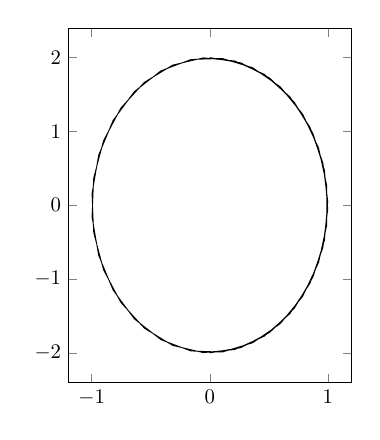
\begin{tikzpicture}[scale = 0.75]
                    \begin{axis}
                    [
                        y=1.25cm,
                        x=2cm,
                        view={60}{30},
                    ]
                    \addplot[
                        domain=0:5*pi,
                        samples = 60,
                        samples y=0,
                    ]
                    ({sin(deg(x))}, {2*cos(deg(x))});
                    \end{axis}
                \end{tikzpicture}
            \end{center}
        \end{wrapfigure}
        \begin{align}
            f(x,y) =& x^2 + \frac{y^2}{4}\\
            \{f(x,y) =& 1\}\text{\;(Level set)}\\
            =& \{(x,y)|x^2 + \frac{y^2}{4} = 1\}
        \end{align}
        Theorem: Given $f(x,y)$ differentiable, then the gradient $\nabla f\perp$ the level set.
        
        We can prove it by using the chain rule: let $\gamma(t)$ be a parametric function of my level set $\{f(x,y) = 1\}$, $f(\gamma(t))=1$ and differentiate both sides.
        \begin{align}
            0 = D(f(\gamma(t))) =& Df(\gamma(t)) D(\gamma(t))\\
            =& \nabla F(\gamma(t))_{1\times2} \cdot (\gamma_1'(t),\gamma_2'(t))_{2\times1}\\
            \text{Hence\;}\Rightarrow& \nabla F(\gamma(t))_{1\times2} \perp (\gamma_1'(t),\gamma_2'(t))_{2\times1}
        \end{align}
        Example: Look at a surface $\sin(xy)-2\cos(yz)=0$ Find the tangent plane of this surface at $(\frac{\pi}{2},1,\frac{\pi}{3})$. The idea is that consider the surface as a level set of $F(x,y,z) = \sin(xy)-2\cos(yz),\{F=0\}$
        
        Using the Theorem: $\nabla F$ is hence perpendicular to this surface, giving us the normal direction of our tangent plane.
        
        \begin{align}
            \nabla F = (\frac{df}{dx},\frac{df}{dy},\frac{df}{dz})
            =& (y\cos(xy),x\cos(xy)+2z\sin(yz),2y\sin(tz))\\
            =& (\cos(\frac{\pi}{2}),\frac{\pi}{2}\cos(\frac{\pi}{2})+\frac{2\pi}{3}\sin(\frac{\pi}{3}),2\sin(\frac{\pi}{3}))\\
            =& (0,\frac{\sqrt{3}\pi}{3},\sqrt{3})\\
            0=&0\cdot(x-\frac{\pi}{2}) + \frac{\sqrt{3}\pi}{3}(y-1)+\sqrt{3}(z-\frac{\pi}{3})
        \end{align}
        Where the last equation above is the equation of the tangent plane.
        
    \subsection{Parametric Curves}
        \dots are vector functions in 1 variable.
        
        Definition: A parametric curve in $\R^n$ is a vector valued function where $\vec{c}(t):R^1\rightarrow\R^n$
        
        All the component functions of $\vec{c}(t)$ are functions in 1 variable.
        
        Example:
        
        1) Draws a Circle
        \begin{align}
            \vec{c}(t) = (\cos(t),\sin(t)),t\in[0,2\pi]
        \end{align}
        2) Draws a eclipse at plane z = 3
        \begin{align}
            \vec{c}(t) = (a\cos(t),b\sin(t),3),t\in[0,2\pi]
        \end{align}
        3) Eclipse spiraling up
        \begin{align}
            \vec{c}(t) = (a\cos(t),b\sin(t),t),t\in[0,2\pi]
        \end{align}
        
        Definition: Orientation of $\vec{c}(t)$, the direction corresponding to increasing t-value is called the positive orientation of $\vec{c}(t)$. The opposite direction is the negative orientation.
        
        Example: Positive orientation = Clockwise
        \begin{align}
            \vec{c}(t) = (\cos(t),-\sin(t),t),t\in[0,2\pi]
        \end{align}
        
        Derivative of $\vec{c}(t)$
        
        If $\vec{c}(t) = (x(t),y(t),z(t))$, $\vec{c'}(t) = (x'(t),y'(t),z'(t))$
        
        \begin{enumerate}
            \item $\vec{c}(t)$ is a vector function
            \item $\vec{c'}(t)$ is a tangent to curve $\vec{c}(t)$
        \end{enumerate}
        
        Terminology: $\vec{c'}(t)$ is the velocity of $\vec{c}(t)$, and $|\vec{c'}(t)|$ is the speed of $\vec{c}(t)$. The speed of the curve $\vec{c}(t) = (\cos(t), \sin(t))$ for example, is 1.\\
        
        What is the length of curve $\vec{c}(t) = (\cos(t),\sin(t),t)$ between (0 to 2$\pi$)Given $\vec{c}(t)$ differentiable between range a and b, length of the curve would be
        
        \begin{align}
            l =& \int^{b}_{a}{|\vec{c'}(t)|}dt\\
            |\vec{c'}(t)| =& \sqrt{\sin(t)^2 + \cos(t)^2 + 1} = \sqrt{2}\\
            l =& \int^{2\pi}_{0}{\sqrt{2}dt}
        \end{align}
        Think of length as a function in t
        \begin{align}
            l(t) = \int^{t}_{a}{|\vec{c'}(x)|}dx
        \end{align}
        If curve $\vec{c}(t)$ differentiable and $\vec{c}(t) \neq 0$,
        \begin{enumerate}
            \item $|\vec{c'}(t)| > 0$
            \item $l(t)$ strictly increasing.
            \item l is one to one function so has inverse.
        \end{enumerate}
        \begin{align}
            l[a,b] \rightarrow& \R^1,\text{\;l has an inverse.}\\
            t\rightarrow& l(t),\text{\;think of our parameter t}\\
        \end{align}
        t can now be expressed as a function in terms of length, $\vec{c}(t) = \vec{c}(t(l)) = \vec{c'}(l)\\$
        
        Proof:
        
        In our last example of calculating length, we can find an inverse for $l(t) = \sqrt{2}t$ resulting $t = \frac{l}{\sqrt{2}}$, by substitution we can reparameterize $\vec{c}(t)$ into $\vec{c}(l)$\\
        
        \begin{align}
            c(l) =& \vec{c}(t(l))\\
            \frac{d\vec{c}(l)}{dl} =& \frac{\vec{c}(t(l))}{dt}\cdot\frac{dt}{dl}\\
            =&\vec{c'}(t)\cdot\frac{1}{|\vec{c'}(t)|}\\
            |\frac{d\vec{c}(l)}{dl}|=&|\vec{c'}(t)|\cdot\frac{1}{|\vec{c'}(t)|}=1
        \end{align}


\end{document}